\documentclass[lualatex,ja=standard]{bxjsarticle}

\setpagelayout{noheadfoot,top=1.5cm,bottom=1.5cm,left=2cm,right=2cm}

% タイトル情報(必要に応じて編集)
\title{タイトル}
\author{著者}
\date{\today}

% パッケージ類
\usepackage{graphicx}   % 画像を挿入するため
\usepackage{amsmath}    % 数式を使うため
\usepackage{amssymb}    % 数式を使うため
\usepackage{caption}    % 図表のキャプション
\usepackage{subcaption} % サブキャプション
\usepackage{siunitx}    % 数式の設定
\usepackage{float}      % 図の配置設定
\usepackage{booktabs}   % 表のスタイル
\usepackage{multirow}   % 表のスタイル
\usepackage{pdfpages}   % 表紙の挿入
\usepackage{enumitem}   % 箇条書き
\usepackage{titlesec}   % セクションのスタイル
\usepackage{luatexja-fontspec} % フォント設定
\usepackage{xspace}     % スタイルの装飾
\usepackage{makecell}   % 表のセルを結合するため
\usepackage{ascmac}     % 図の枠を作成するため
\usepackage{listings}   % ソースコードの表示
\usepackage{comment}    % コメントの使用
\usepackage{fancyhdr}   % ヘッダー・フッター

\usepackage{hyperref}   % 図表へのリンク

% フォント
\setmainjfont{IPAexMincho} 
\AtBeginDocument{%lst
  \fontsize{10.5pt}{16pt}\selectfont
}

% 樹形図
\usepackage{tikz}
\usetikzlibrary{graphs, graphdrawing, arrows.meta, calc}
\usegdlibrary{trees}  % trees 用ライブラリ

% セクションスタイル
\newcommand{\mysectionstyle}[2]{%
  \sffamily         % 欧文・数字→サンセリフ
  \gtfamily         % 日本語→ゴシック
  \bfseries
  \fontsize{#1}{#2}\selectfont
}

% セクションのスタイル
\titleformat{\section}
  {\mysectionstyle{12pt}{16pt}}
  {\mysectionstyle{12pt}{16pt}\thesection.}
  {0.7em}{}
\titlespacing*{\section}{0em}{1em}{0em}

% サブセクションのスタイル
\titleformat{\subsection}
  {\mysectionstyle{10.5pt}{16pt}}
  {\mysectionstyle{10.5pt}{16pt}\thesubsection.}
  {0.7em}{}
\titlespacing*{\subsection}{0em}{0.5em}{0em}

% サブサブセクションのスタイル
\titleformat{\subsubsection}
  {\mysectionstyle{10.5pt}{12pt}}
  {\mysectionstyle{10.5pt}{12pt}\thesubsubsection.}
  {0em}{}
\titlespacing*{\subsubsection}{0em}{0.5em}{0em}

% パラグラフのスタイル
\titleformat{\paragraph}
  {\mysectionstyle{10.5pt}{12pt}}
  {\mysectionstyle{10.5pt}{12pt}\theparagraph.} 
  {0em}{}
\titlespacing*{\paragraph}{0em}{0em}{0em}

% サブパラグラフのスタイル
\titleformat{\subparagraph}
  {\mysectionstyle{8pt}{12pt}}
  {\mysectionstyle{8pt}{12pt}\thesubparagraph.}
  {0em}{}
\titlespacing*{\subparagraph}{0em}{0em}{0em}

% 和文キャプション
\renewcommand{\figurename}{図}
\renewcommand{\tablename}{表}
\renewcommand{\refname}{参考文献}
\renewcommand{\lstlistingname}{ソースコード}

% autoref の和文化
\renewcommand*{\figureautorefname}{図}
\renewcommand*{\tableautorefname}{表}
\renewcommand*{\equationautorefname}{式}
\renewcommand*{\subfigureautorefname}{図}

\captionsetup[subfigure]{labelformat=simple}
\renewcommand*{\thesubfigure}{(\alph{subfigure})}

\captionsetup[subtable]{labelformat=simple}
\renewcommand*{\thesubtable}{(\alph{subtable})}

% ブラケット付き単位の設定
\NewDocumentCommand{\sibr}{m}{\,\text{[\si{#1}]}}

% ソースコード用の設定
\lstset{
  basicstyle={\ttfamily},
  identifierstyle={\small},
  commentstyle={\small\textnormal},
  keywordstyle={\small\bfseries},
  keepspaces=true,
  ndkeywordstyle={\small},
  stringstyle={\small\ttfamily},
  frame={tb},
  breaklines=true,
  columns=[l]{fullflexible},
  %columns=fixed, % 文字幅を合わせる
  numbers=left,
  xrightmargin=0em,
  xleftmargin=3em,
  numbersep=1em,
  numberstyle={\scriptsize},
  stepnumber=1,
  lineskip=-0.5ex
}

% リンクの色設定
\hypersetup{
  colorlinks=true,
  linkcolor=black,
  citecolor=black,
  urlcolor=black
}

% 参考文献の設定
\usepackage[backend=biber,style=numeric,sorting=none]{biblatex}
\addbibresource{refs.bib}

% アクセス日の表示を和文スタイルに
\DeclareFieldFormat{urldate}{,参照日:#1}

% 参考文献の書式設定
\DeclareDelimFormat{multinamedelim}{,}
\DeclareDelimFormat{finalnamedelim}{,}
\DeclareDelimFormat{nameyeardelim}{,}
\DeclareFieldFormat{title}{#1}
\DeclareFieldFormat{journaltitle}{#1}
\renewcommand*{\newunitpunct}{,}
\DeclareCiteCommand{\cite}
  {\usebibmacro{prenote}}
  {\mkbibsuperscript{[\printfield{labelnumber}]}}
  {\multicitedelim}
  {\usebibmacro{postnote}}

% 書籍フォーマット
\DeclareBibliographyDriver{book}{%
  \printnames{author}:%
  \printfield{title},%
  \printfield{pages},%
  \printlist{publisher} (\printfield{year})%
  \finentry
}

% 雑誌論文フォーマット
\DeclareBibliographyDriver{article}{%
  \printnames{author}:“%
  \printfield{title},”\ %
  \printfield{journaltitle},%
  \printfield{volume},%
  \printfield{pages}(\printfield{year})%
  \finentry
}

% 参照日
\DeclareFieldFormat{urldate}{%
  ,参照日:\thefield{urlyear}/\thefield{urlmonth}/\thefield{urlday}\isdot
}

% 段落設定
\setlength{\parskip}{0.5em}
\setlength{\parindent}{1em}
\makeatletter
\AtBeginDocument{
  \let\@afterindentfalse\@afterindenttrue
}
\makeatother

% ヘッダーとフッター設定
\pagestyle{fancy}  % ページスタイルを変更
\fancyhf{}  % デフォルトのヘッダー・フッターをクリア
\renewcommand{\headrulewidth}{0pt} % ヘッダーの横線を削除
\fancyfoot[C]{\thepage}  % ページ番号を中央下に配置

\begin{document}

% 表紙(wordから出力した表紙をcover/cover.pdfに保存)
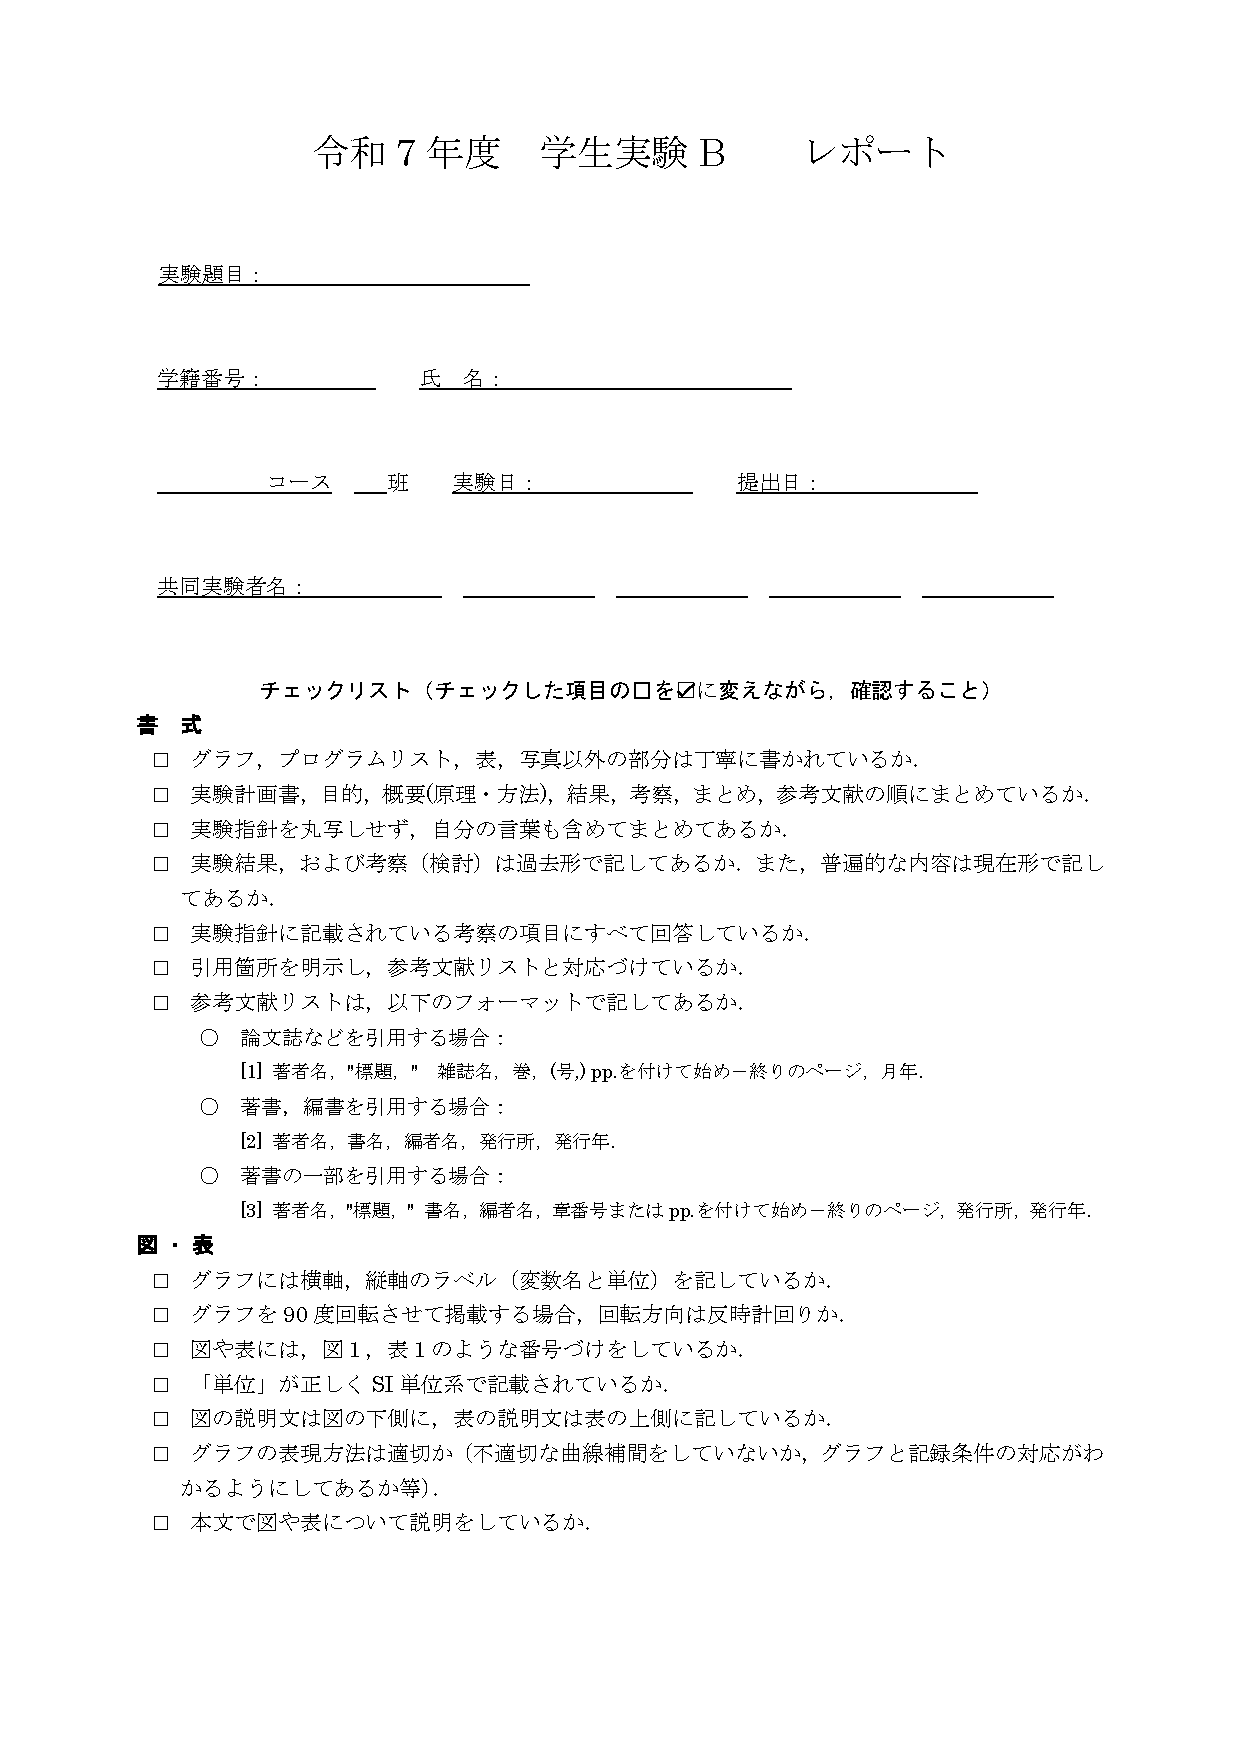
\includepdf[pages=1]{cover/cover.pdf}

% ページ番号をリセット
\pagenumbering{arabic}
\setcounter{page}{1}


\section{実験の目的}


\section{原理}
\subsection{サブセクション1}

\begin{itemize}
\item ネットワーク層
\setlength{\parindent}{1em}



\vspace{1em}
\item トランスポート層(TCP,UDP)
\setlength{\parindent}{1em}



\end{itemize}


\begin{lstlisting}[language=C]
// プログラムコード

\end{lstlisting}


\begin{comment}
\section{実験の方法}
\subsection{サブセクション1}


\subsection{サブセクション2}


\subsection{サブセクション3}


\section{実験結果}
\subsection{サブセクション1}

\begin{table}[H]
  \centering
  \caption{測定結果の例}
  \label{table:1}
  \begin{tabular}{c|cccc}
  \hline
       & 時間 $t$ [\textmu s] & 距離 $x$ [\textmu m] & 電圧値 $V$ [mV] \\
  \hline
  サンプル1     & 10           & 2.0            & 1.6       \\
  サンプル2     & 20           & 3.0            & 7.4       \\
  サンプル3     & 30           & 2.0            & 5.4       \\
  サンプル4     & 40           & 3.0            & 2.0       \\
  サンプル5     & 50           & 3.0            & 4.8       \\
  \hline
  \end{tabular}
\end{table}

\subsection{サブセクション2}


\subsection{サブセクション3}

\section{考察}
\subsection{サブセクション1}


\subsection{サブセクション2}


\subsection{サブセクション3}

\section{結論}
\end{ccomment}

\begin{comment}
\begin{figure}[H] % 横並び
  \centering
  \begin{minipage}[b]{0.48\textwidth}
    \centering
    \includegraphics[width=0.8\textwidth]{img/2.jpg}
    \caption{実験装置1}
    \label{fig:2}
  \end{minipage}
  \hfill
  \begin{minipage}[b]{0.48\textwidth}
    \centering
    \includegraphics[width=0.8\textwidth]{img/3.jpg}
    \caption{実験装置2}
    \label{fig:3}
  \end{minipage}
\end{figure}

\begin{figure}[htbp]% (a)と(b)で横並び
  \centering
  \begin{subfigure}[b]{0.48\textwidth}
    \centering
    \includegraphics[scale=0.8]{img/4-a.jpg}
    \caption{実験回路1}
    \label{fig:4-a}
  \end{subfigure}
  \hfill
  \begin{subfigure}[b]{0.48\textwidth}
    \centering
    \includegraphics[scale=0.8]{img/4-b.jpg}
    \caption{実験回路2}
    \label{fig:4-b}
  \end{subfigure}
  \caption{横に並べた図の例}
  \label{fig:4-b}
\end{figure}
\end{comment}

\printbibliography[title=<参考文献>]

\end{document}
